\begin{section}{Datenbankmodell}

\subsection{ER-Model}
Nach Analyse der Anforderungen, wurde das nachfolgende Domainmodell entworfen.
Zusätzlich zu den vorgegebenen Entitäten (user, artist, ...), werden noch zwei weitere benötigt: Location und Country.
Da es möglich ist, dass an einer Location (z.B. Landhaus, Hauptplatz...) mehrere Spielstätten (Venues) existieren, wird durch auslagern der Information in eine eigene Entität Datenredundanz vermieden.
\\

Für die konkrete Implementierung, wurde in Erwin das Schema entworfen per ForwardEngineering an eine MySQL Datenbank exportiert. Diese wird über phpMyAdmin verwaltet und die SQL-Scripte wurden nachträglich via Exportfunktionalität von MySQL generiert.
\\

Die Primärschlüssel (IDs) der Entitäten User, Location und Artist werden in der Datenbank per Auto-Incrementation automatisch nummeriert. \\

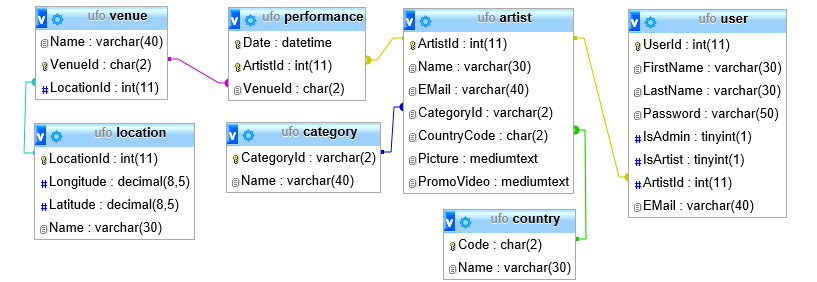
\includegraphics[angle=0, scale=0.45]{./img/databaseEntities.jpg}
\FloatBarrier

\subsection{Performance}
Um Aufführungen eindeutig abbilden zu können, wurde eine Primärschlüssel-Beziehung zwischen Artist und Venue in der Performance Entität erstellt. Diese bilden eine eindeutige Abbildung zu welcher Zeit und an welchem Ort ein Artist aufführt. Durch die Überprüfung der Zeit vor einfügen eines Datensatzes wird sichergestellt, dass ein Artist nicht eine Stunde vor bzw. nach seinem Auftritt wieder eingetragen werden kann.

\subsection{User}
Die Stammdatenverwaltung der User beinhaltet eine Referenz auf ein Artist Objekt, welches impliziert, dass der User nicht nur administrative Funktionalitäten beinhalten kann, sondern auch selbst als Artist funktionieren kann.
Wenn ein User auch ein Artist ist, wird das Flag IsArtist = 1 gesetzt.
Ein User kann auch als Admin deklariert werden mit IsAdmin = 1. Das heißt, er kann beide Eigenschaften beinhalten.
Diese Abbildung bildet die Basis für eine mögliche Erweiterung der Anwendung, wo sich User, die einem Artisten zugeordnet sind, einloggen können und Stammdaten wie Foto oder Promovideo selbst künftig ändern könnten.

\subsection{Artist}
Für Picture und PromoVideo werden Links in Form eines Strings in der Entität abgebildet. Die Pictures werden in einem BlobData Objekt abgeblidet, welches Meta-Informationen wie Name oder Pfad beinhaltet. Dieses Objekt ist serialisierbar und beinhaltet den Binärdatenstrom, welcher bis zum Client ins Frontend durchgetragen werden kann. \\

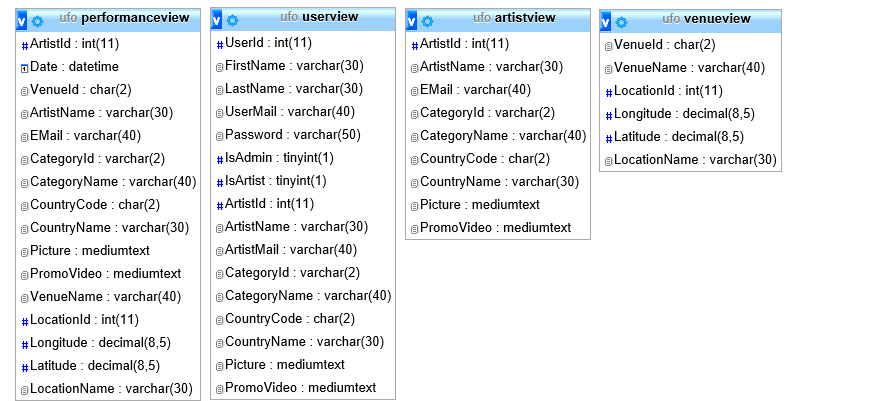
\includegraphics[angle=0, scale=0.45]{./img/databaseViews.jpg}
\FloatBarrier

\nPar

Des Weiteren werden vier Sichten erstellt: Performance-View, User-View, Artist-View und Venue-View. Dadurch können alle zusammenhängenden Daten mit einer Abfrage geladen werden und das verhindert Join-Statements im C\# Code.
Der wesentliche Vorteil besteht darin, dass gegebenenfalls alle benötigten Objekte mit einer Abfrage instanziiert werden können, wo ansonsten (wie im folgenden Beispiel) drei Anfragen an die Datenbank benötigt würden.

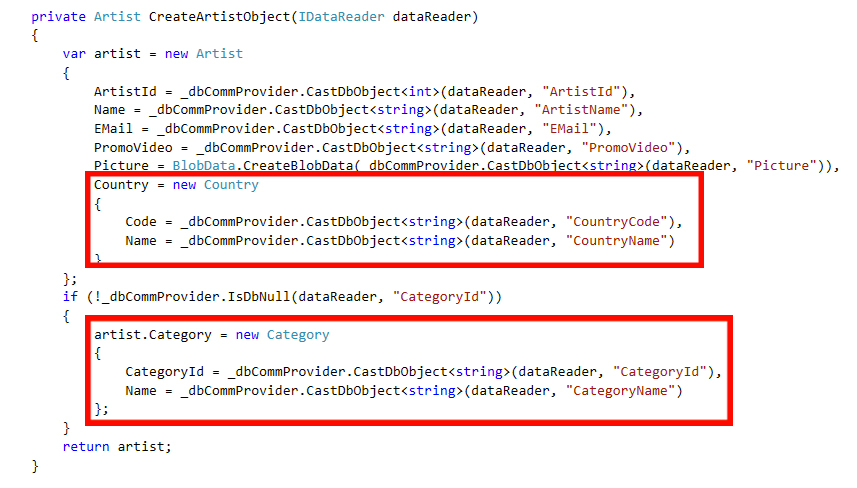
\includegraphics[angle=0, scale=0.45]{./img/viewcodesample.jpg}
\FloatBarrier

Zusätzlich um Nullwerte aus der Datenbank unterscheiden zu können und zum richtigen Datentyp mappen zu können, werden alle DataReader Zugriffe über die CastDbObject<T> Methode delegiert. Diese sorgt bei Nullwerten für den richtigen Standardwert.\\

\textbf{Die Daten in der Datenbank stammen von:} \\
User: \\ \url{http://convertcsv.com/generate-test-data.htm} \\
Country: \\ \url{http://blog.plsoucy.com/wp-content/uploads/2012/04/countries-20140629.csv} \\
Artist, Venue, Category, Location: \\ \url{http://www.pflasterspektakel.at/2015/de/1443.asp} (wurden manuell mit Excel angepasst) \\
Die jeweiligen SQL Scripten, wurden im Verzeichnis UFO.Database/sql bereitgestellt.


\end{section}